% Question 1
\begin{enumerate}
    \item (10 points) Find the domain and the inverse of the following functions:
    \begin{enumerate}
        \item \( f(x) = \frac{x^5}{5} - 1 \)
        \item \( y = 3 - \sqrt{x} \)
        \item \( y = \ln(x + 2) \)
    \end{enumerate}

% Question 2
\item (10 points)
\begin{enumerate}
    \item[(a)] (4 pts) Find the equation of the vertical asymptotes \(x = a\) of the function:  
    \[
    f(x) = \frac{x^2 + 2}{x^2 - 7x + 10}
    \]
    \item[(b)] (6 pts)Using the graph of function \( f(x) \) given below, answer the following questions.
        (If a limit does not exist, write “DNE” and if function is undefined at a point, write “undefined”.)
    \begin{figure}[ht!]
        \centering
        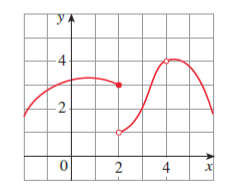
\includegraphics[width=0.35\linewidth]{/Users/melusi/Desktop/Projects/COSC 4315 Project/exam_collection/E1C1Q2b_graph.png}
    \end{figure}

<<<<<<< HEAD
=======
% Question 3
    \item (6 pts) Using the graph of function \( f(x) \) (provided in the original exam), answer:
>>>>>>> c4e0eda185b991e902176d73ee63844cffd9f303
        \begin{enumerate}
            \item \( \lim_{x \to 2^-} f(x) = \)
            \item \( \lim_{x \to 2^+} f(x) = \)
            \item \( \lim_{x \to 2} f(x) = \)
            \item \( f(2) = \)
            \item \( \lim_{x \to 4} f(x) = \)
            \item \( f(4) = \)
        \end{enumerate}
    \end{enumerate}

<<<<<<< HEAD
% Question 3
=======
% Question 4
>>>>>>> c4e0eda185b991e902176d73ee63844cffd9f303
    \item (10 points)
    \begin{enumerate}
        \item [(a)] (5 pts) Determine the infinite limits:
        \[
        \lim_{x \to 2^+} \frac{x + 1}{x - 2}, \quad 
        \lim_{x \to 4^-} \frac{x}{x - 4}
        \]

        \item [(b)] (5 pts) Find \( f \circ g \circ h \) for the functions: \\
        \( f(x) = 2x + 1,\ g(x) = x^2,\ h(x) = \cos x \)
    \end{enumerate}

<<<<<<< HEAD
% Question 4
=======
% Question 5
>>>>>>> c4e0eda185b991e902176d73ee63844cffd9f303
    \item (10 points)
    \begin{enumerate}
        \item [(a)]  (5 pts) Solve:
        \[
        x = \log_2 8 + \log_2 \left(\frac{1}{8}\right) + \ln e
        \]

        \item [(b)] (5 pts) Evaluate the limit and find the horizontal asymptotes:
        \[
        \lim_{x \to \infty} \frac{3x^2 - 5x + 2}{4 - 3x - x^2}
        \]
    \end{enumerate}

<<<<<<< HEAD
% Question 5
=======
% Question 6
>>>>>>> c4e0eda185b991e902176d73ee63844cffd9f303
    \item (10 points) Evaluate the following limits algebraically:
    \begin{enumerate}
        \item [(a)]  \( \lim_{x \to 3} \frac{x^2 - 9}{x^2 - 4x + 3} \)
        \item [(b)] \( \lim_{x \to 0} \frac{(x - 1)^2 - 1}{x} \)
    \end{enumerate}

<<<<<<< HEAD
% Question 6
=======
% Question 7
>>>>>>> c4e0eda185b991e902176d73ee63844cffd9f303
    \item (10 points) Determine if \( f \) is continuous or discontinuous at the given points. If discontinuous, choose one of: 
    (i) \( f \) is undefined, 
    (ii) limit does not exist, 
    (iii) \( \lim_{x \to a} f(x) \neq f(a) \)

    \begin{figure}[ht!]
        \centering
        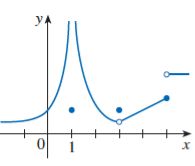
\includegraphics[width=0.35\linewidth]{/Users/melusi/Desktop/Projects/COSC 4315 Project/exam_collection/E1C1Q6_graph.png}
    \end{figure}

    \begin{itemize}
        \item [(a)] At \( x = 1 \)
        \item [(b)] At \( x = 2 \)
        \item [(c)] At \( x = 3 \)
        \item [(d)] At \( x = 4 \)
        \item [(e)] At \( x = 5 \)
    \end{itemize}

<<<<<<< HEAD
 % Question 7
=======
 % Question 8
>>>>>>> c4e0eda185b991e902176d73ee63844cffd9f303
    \item (10 points) Let \( f(x) = x^2 + 3 \)
    \begin{enumerate}
        \item [(a)] Find the derivative \( f'(x) \) using the limit definition.
        \item [(b)] Use \( f'(x) \) to find the slope of the tangent line to the curve at \( x = 1 \).
    \end{enumerate}

<<<<<<< HEAD
% Question 8
=======
% Question 9
>>>>>>> c4e0eda185b991e902176d73ee63844cffd9f303
    \item[\textbf{Bonus.}] (10 points)
    \begin{enumerate}
        \item Find the value of constant \( c \) so that the function is continuous everywhere:
        \[
        G(x) = 
        \begin{cases}
            4 - \cos x, & x < 0 \\
            \sqrt{x + 3c}, & x \geq 0
        \end{cases}
        \]

        \item Find the horizontal and vertical asymptotes of:
        \[
        f(x) = \frac{2e^x}{e^x - 5}
        \]
    \end{enumerate}
\end{enumerate}
